\section{Systemarkitektur}
Systemet er opbygget af tre forskellige delsystemer samt et delt kodebibliotek iht. ovenstående afsnit \ref{section:specanal}. De tre delsystemer, Administrationssystem, Kasseapparat og CentralServer, benytter alle delt funktionalitet i kodebiblioteket SharedLib.\\

Mellem de tre delsystemer kommunikeres via en TCP/IP~\cite{TCPIP} socket-forbindelse.

\begin{figure}[H]
    \centering
    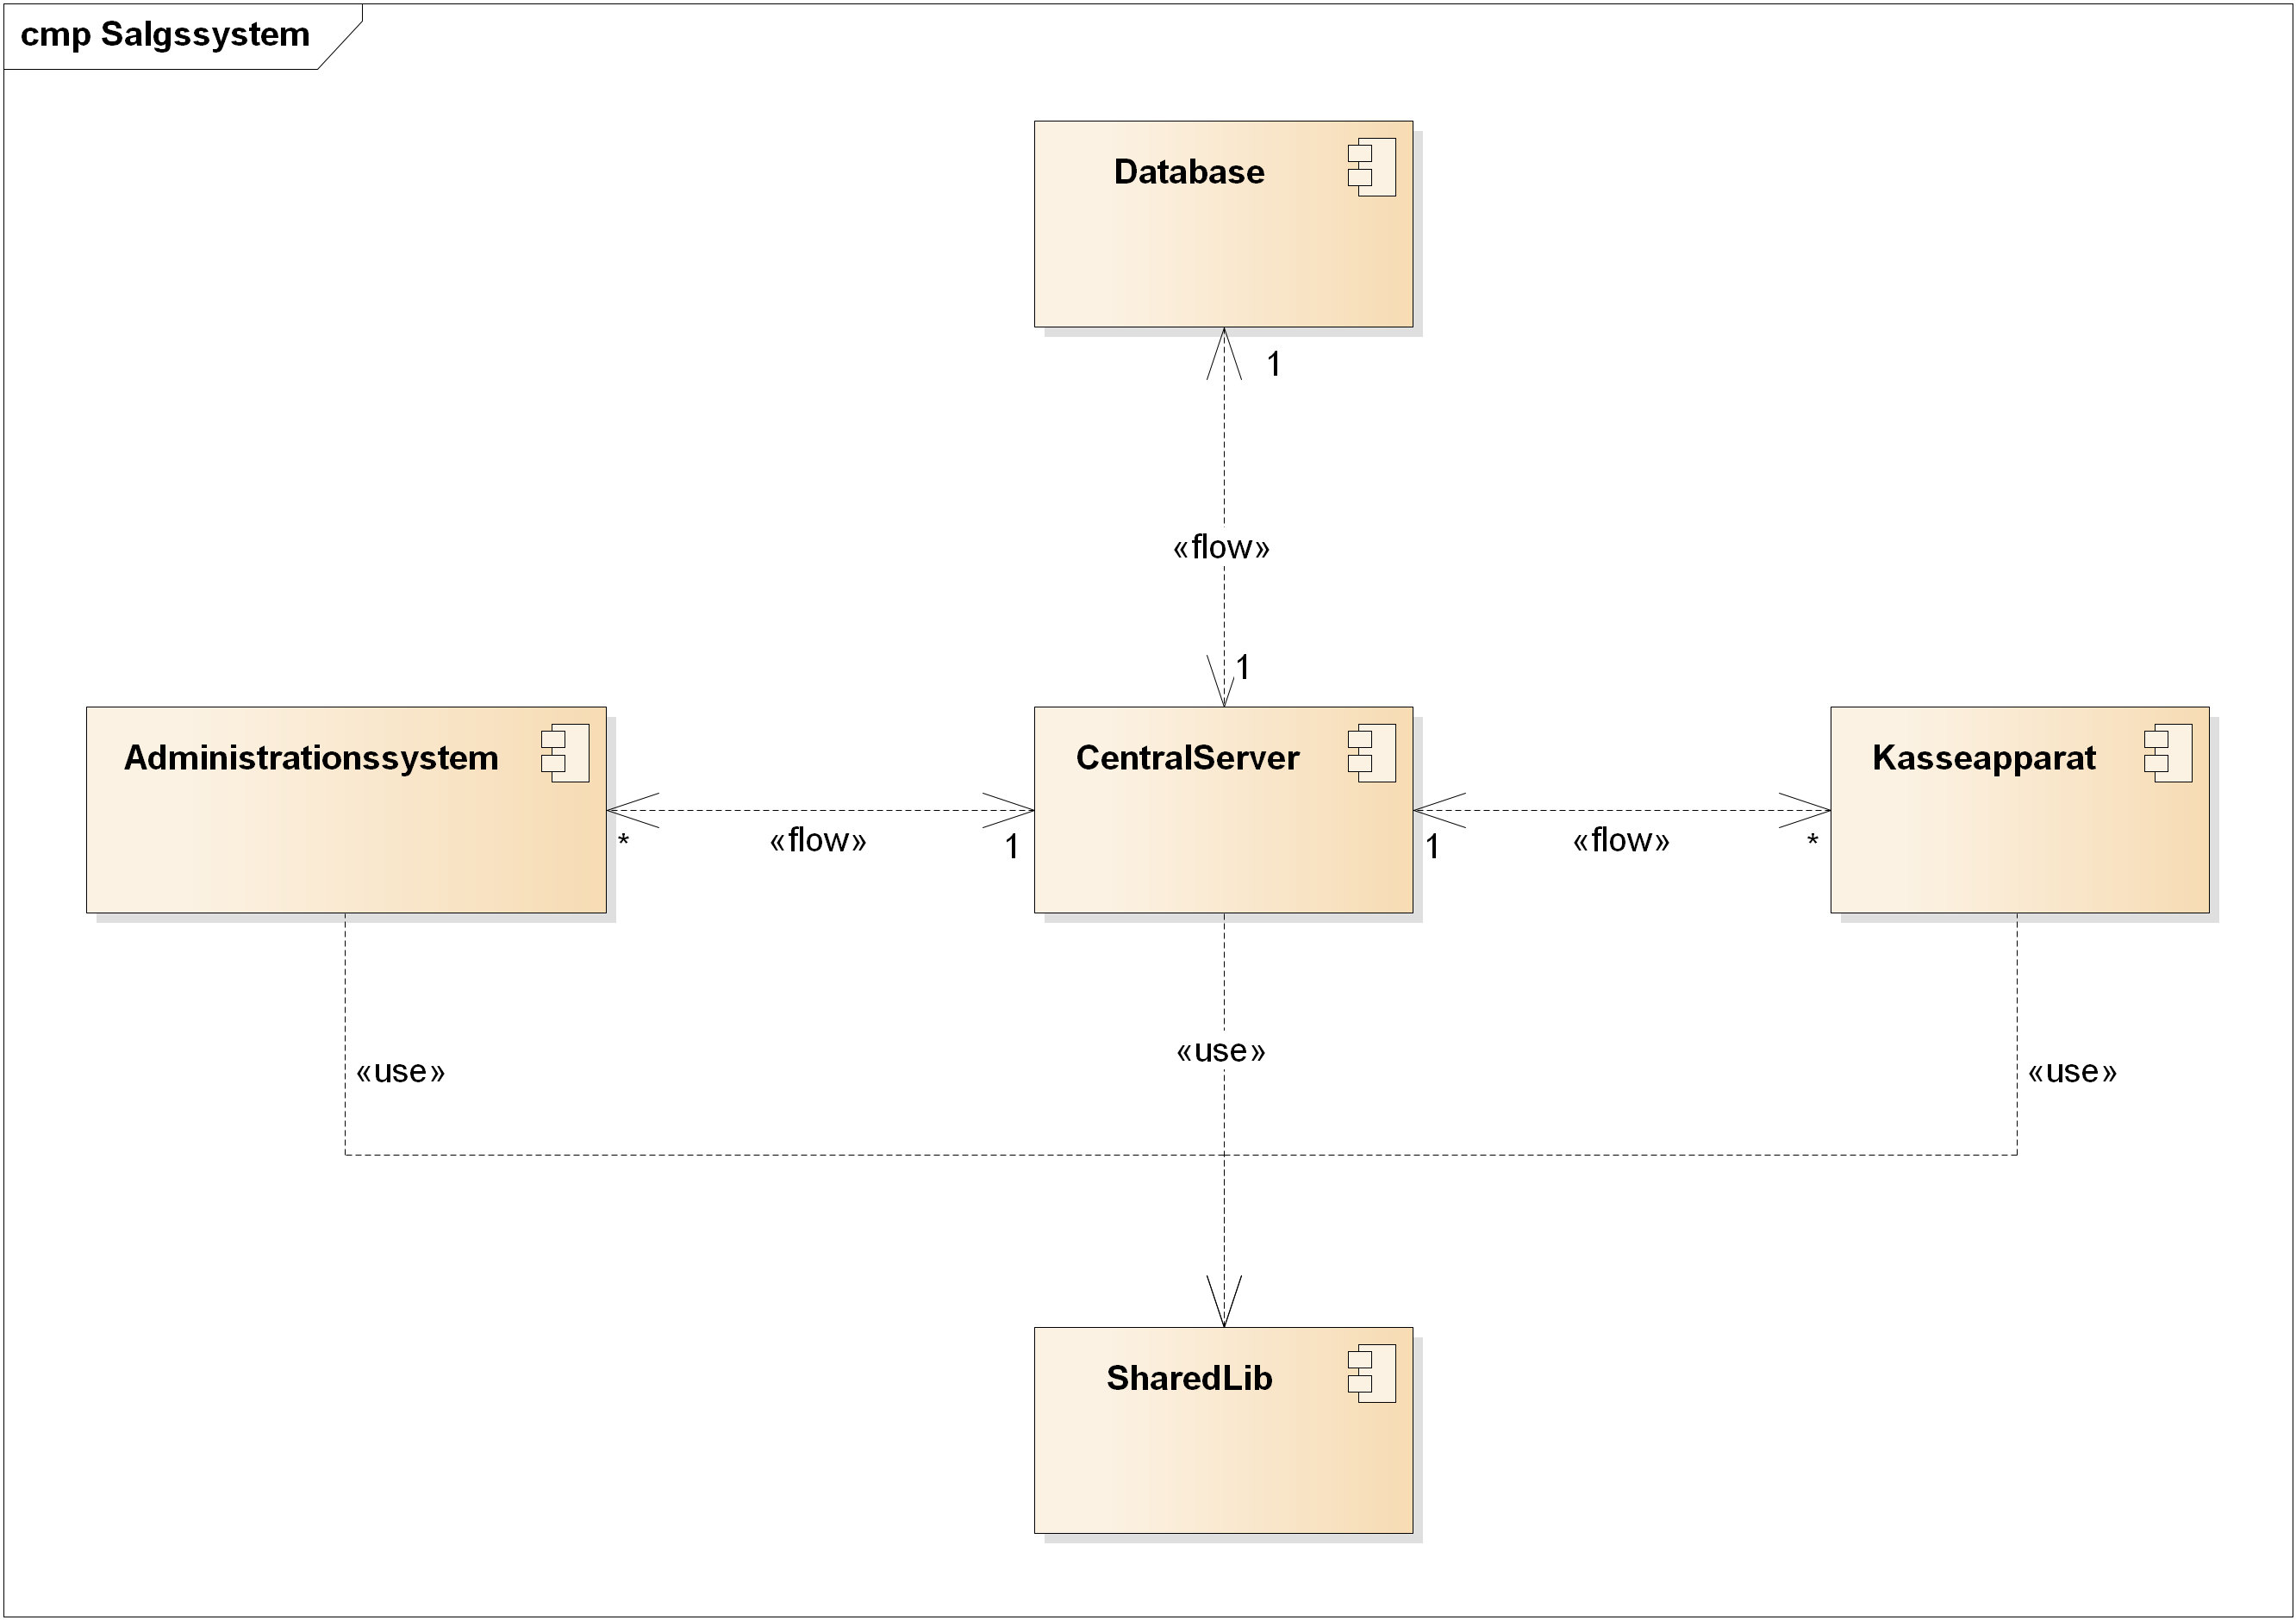
\includegraphics[width=1\textwidth]{Projektbeskrivelse/Systemarkitektur/Components.png}
    \caption{Component diagram for samtlige delsystemer i Salgssystem}
    \label{fig:CSLogging}
\end{figure}


\textbf{SharedLib}\\
SharedLib indeholder den funktionalitet, som er delt på tværs af de andre tre delsystemer. Denne funktionalitet compiles til en DLL-fil\footnote{Dynamic-Link Library fil}, som kan inkluderes i de andre projekter.\\

SharedLib indeholder kommunikationsprotokol, datamodeller samt en klasse til at implementere en asynkron socket-klient.\\

\textbf{Administrationssystem}\\
Administationssystemet er den del af systemet som administrerer produkter og produktkategorier. Denne benytter SharedLib's funktionalitet i form af datamodeller samt en socketforbindelse, hvor igennem kommunikkerer med CentralServer.\\


\textbf{Kasseapparat}\\
Kasseapparatet er den del af systemet som er repræsenteret i selve butikken. Det er igennem Kasseapparat, at Ekspedient håndterer salg og returneringer af produkter. \\

\textbf{CentralServer}\\
CentralServer er bindeleddet mellem Administrationssystem, Kasseapparat og Database. Den stiller en socket-server til rådighed, hvor en eller flere klienter kan forbindes til, og kommunikere med, asynkront.\\

CentralServer er det eneste delsystem, der kommunikerer direkte med Database. Administrationssystem og Kasseapparat kommunikerer derfor indirekte med Database gennem CentralServer.\\

CentralServer sørger for at transmittere opdateringer når det er nødvendigt. Eksempelvis får alle forbundne klienter besked når der oprettes et nyt produkt.\\

\textbf{Database}\\
I projektet benyttes en MSSQL\footnote{Microsoft SQL server} server til at opbevare persistent data.
